\documentclass[a4paper]{jsarticle}
\usepackage[all]{xy}
\usepackage[dvipdfmx]{graphicx}
\usepackage{mathtools}
\usepackage{../math_note, exercise, enumitem}
\renewcommand{\thesection}{Ex7.\arabic{section}}

\newcommand{\coverU}{\mathfrak{U}}
\newcommand{\coverV}{\mathfrak{V}}

\newcommand{\Div}{\operatorname{Div}}
\newcommand{\Cl}{\operatorname{Cl}}
\newcommand{\CaCl}{\operatorname{CaCl}}
\newcommand{\nullCaCl}{\operatorname{CaCl}^{0}}
\newcommand{\Pic}{\operatorname{Pic}}

\newcommand{\Sym}{\operatorname{Sym}}
\newcommand{\pbundle}{\mathbb{P}}
\begin{document}
    以下での($*$)とは,次のもの:
    \begin{itemize}
        \item integral,
        \item separated,
        \item noetherian, and
        \item regular in codimention one.
    \end{itemize}

    また,($\dagger$)は次のもの:
    $X$ :: noetherian scheme, 
    $\shS$ :: graded $\shO_X$-algebra
    となっている.
    また,$d \in \Z, d \geq 0$について,
    $\shS_d$ :: homogeneous part of $\shS$を$U \mapsto \shS(U)_d$.
    $X,\shS$は次をすべて満たす.
    \begin{itemize}
        \item $\shS$ :: quasi-coherent.
        \item $\shS=\bigoplus_{d \geq 0} \shS_d$.
        \item $\shS_0=\shO_X$.
        \item $\shS_1$ :: coherent $\shO_X$-module.
        \item $\shS$ :: locally generated by $\shS_1$ as $\shO_X$-algebra.
    \end{itemize}

\section{Surjective Mophism between Invertible Sheaves is Isomorphic.} %% Ex7.1 
    $X$ :: locally ringed space,
    $\shL, \shM$ :: invertible sheaves on $X$,
    $f: \shL \to \shM$ :: surjective mophism,
    とする.
    
    \paragraph{Proof 1.}
    任意の点$x \in X$をとり,$A=\shO_{X,x}$とおく.
    $f_x: \shL_x \to \shM_x$は同型写像を合成することで
    $\phi: A \to A$ :: surjective $A$-morphismと同一視出来る.
    $\phi$ :: surjectiveより,
    $\phi(\alpha)=1 \in A$となる$\alpha \in A$がとれる.
    また$\phi$は$A$-module morphismだから,$\alpha \phi(1)=1$.
    そこで$\psi: A \to A$を$a \mapsto \alpha a$と定義すれば,
    これが$\phi$の逆写像になる.
    よって$\phi, f_x$は同型.
    Prop1.1から,$f$ :: iso.

    \paragraph{Proof 2.}
    Matsumura, Thm2.4から分かる.
    これはNAK (or Nakayama's Lemma)からの帰結である.

    \begin{Remark}
        $k(x)$ :: residue fieldと
        $f_x: \shL_x \to \shM_x$をテンソルすると,
        $f_x \otimes \id{k(x)}$ :: surjective $k(x)$-module morphismが得られる.
        よって$\ker (f_x \otimes \id{k(x)})=0$.
        しかし,ここからNAKをつかって$\ker f_x=0$を導くことは出来ない.
        $k(x)$がflat $\shO_{X,x}$-moduleでなく,
        したがって$\ker (f_x \otimes \id{k(x)})$と$(\ker f_x) \otimes k(x)$の間に同型があることが
        言えないからである.
        このことはflat $\implies$ torsion-freeに気をつければすぐに分かる.
        同様の議論が$f_x$ :: injective(と$\coker f_x$)の場合に出来ることにも気づくが,
        このときは$\Z_2 \to \Z_2; 1 \mapsto 3$という反例がある.
    \end{Remark}

\section{Two Sets of Global Generators and Corresponding Morphisms.} %% Ex7.2 
    $k$ :: field,
    $X$ :: scheme /$k$,
    $\shL$ :: invertible sheaf on $X$,
    $S=\{s_0,\dots,s_m\}, T=\{t_0,\dots,t_n\}$ :: global generators of $\shL$.
    とする.
    ここで$S,T$は
    同じ線形(部分)空間$V \subseteq \Gamma(X, \shL)$を張るとする.
    また$n \leq m, d=\dim_k V$とする.

    $S,T$からそれぞれThm7.1のように定まるmorphismを$\phi_S, \phi_T$とする.
    $\phi_S$が次のように分解できることを示す.
    \[
        \xymatrix
        {
            X \ar@/_20pt/[rrrr]_-{\phi_S}\ar[r]^-{\phi_T}&
                \im \phi_T \ar@{^{(}->}[r]& \proj^m-L \ar[r]^-{\pi}&
                    \proj^n \ar[r]^-{\alpha}& \proj^n
        }
    \]
    ここで$\pi, \alpha$はそれぞれlinear projectionとautomorphismである.

    $X \to \proj^n$のmorphismを考えることは,
    $k[y_0,\dots, y_n]$の元$y_0,\dots,_n$の変換を考えることと同じである.
    これはThm7.1の証明を観察すれば分かる.
    二つの$k$-linear mapは$\phi_S^*, \phi_T^*$はそれぞれ,
    $y_i \mapsto s_i (i=0,\dots,n)$,
    $y_i \mapsto t_i (i=0,\dots,m)$で定まっている.
    したがって問題は,
    $t_0,\dots,t_m$を$s_0,\dots,s_n$へ
    変換するprojectionとautomorphismをつくる問題,
    と言い換えられる.

    今,次のような$(m+1) \times (n+1)$行列$Q$が存在する.
    \[
        \tatev{ s_0 \\ \vdots \\ s_n }
        =Q \tatev{ t_0 \\ \vdots \\ t_m }.
    \]
    $S,T$が$V$の生成系であることから$\rank Q=\dim V=:d$.
    $Q$は基本行列をいくつもかける(あるいは基本変形を繰り返し行う)ことにより,
    次の形に分解できる.
    \[
        Q=L P_{d} R~~
        \mwhere~ L \in PGL(m,k), R \in PGL(n,k)
    \]
    ただし行列$P_r ~(r=1,\dots,n+1)$は$r \times r$-identity matrix $I_r$をもちいて
    $P_{r}=
    \begin{bmatrix}
        I_r & 0 \\
        0 & 0
    \end{bmatrix}$
    と定義される行列である.
    (TODO: $P_{d}$を$P_{n+1}$に交換しても問題ない?)
    $L, P_{n+1}, R$が誘導するmorphismをそれぞれ$\beta, \tilde{\pi} ,\alpha$とすれば,
    $\alpha, \beta$はautomorphismであり,
    $\tilde{\pi}$はprojectionである.
    \[
        \xymatrix
        {
            \proj^m \ar[r]^-{\beta}& \proj^m
            \ar@{^{(}->}[r]^-{i}& \proj^m-L
            \ar[r]^-{\tilde{\pi}}& \proj^n
            \ar[r]^-{\alpha}& \proj^n
        }
    \]
    求める射はこの$\alpha$と,$\pi=\beta \circ i \circ \tilde{\pi}$である.
    また,$L=\zerosp(y_0,\dots,y_n) \subseteq \proj^m$の次元は$m-(n+1)$である.

\section{Morphism of $\proj^n \to \proj^m$ can be Decomposed into Common Ones.} %% Ex7.3
    $\phi: \proj^n_k \to \proj^m_k$を考える.
    $\shO_{\proj^m}(1), \shO_{\proj^n}(1)$
     :: invertible sheaves
    のglobal generatorをそれぞれ
    $\{x_0,\dots,x_m\}, \{y_0,\dots,y_n\}$
    とする.

    \subsection{$\im \phi=pt$ or $m \geq n$ and $\dim \im \phi=n$.}
%    $\eta: \Gamma(\proj^m, \shO_{\proj^m}(1)) \to \Gamma(\proj^m, \phi^* \phi_* (\shO_{\proj^m}(1)))$を
%    adjoint pair $\phi^* \dashv \phi_*$のunitから得られる射とする.
%    これが本文中で$\phi^*$と表記されているものである
    $s_i=\phi^*(x_i)~(i=0,\dots,m)$とおくと,
    $s_0,\dots,s_m$は$\shL:=\phi^*(\shO_{\proj^m}(1))$のglobal generatorである.
    $\shL$は$\proj^n$上のinvertible sheafだから,
    Cor6.17より,$\shL \iso \shO_{\proj^n}(d)$となる$d \in \Z$が存在する.
    Example7.8.3同様,$\shO_{\proj^n}(d)$は$|d|$次斉次単項式で生成される.

    \paragraph{$m<n \implies \dim \im \phi=0$.}
    \paragraph{$m \geq n \implies \dim \im \phi=n$.}

\section{If $X$ Admits an Ample Invertible Sheaf, then $X$ is Separated.} %% Ex7.4
    \subsection{Assumption of Thm7.6 $\implies$ $X$ :: separated.}
    $A$ :: noetherian ring,
    $X$ :: scheme of finite type /$A$とする.
    $\shL$ :: ample invertible sheaf on $X$が存在したとする.
    Thm7.6から,immersion $i: X \to \proj^n_A ~(n>0)$が存在する.
    これは$X$から$\proj^n_A$のlocally closed subschemeへのisomorphismである.
    これにprojection $\pr: \proj^n_A=\proj^n_{\Z} \times_{\Z} \Spec A \to \Spec A$を
    合成したものは,quasi-projective.
    \[\xymatrix
    {
        X \ar[r]^-{\sim}& U ~\ar@{^{(}->}[r]& Z ~\ar@{^{(}->}[r]& \proj^n_A \ar[r]^-{\pr}& \Spec A
    }\]
    $Z$は$\proj^n_A$のclosed subscheme,
    $U$は$Z$のopen subschemeである.
    $A,X$についての仮定から$\Spec A, X$ :: noetherian schemeがわかる
    \footnote
    {
        $f: X \to \Spec A$がfinite typeならば
        $f^{-1}\Spec A=X$はfinite affine open coverをもち,
        各affine open coverはfinitely generated $A$-algebraの$\Spec$である.
        finitely generated $A$-algebraは$A$からnoetherianを受け継ぐから,
        $X$ :: noetherian.
    }
    から,
    Thm4.9より,この射$X \to \Spec A$はseparated.
    
    \subsection{There is No Ample Invertible Sheaf on 
        \protect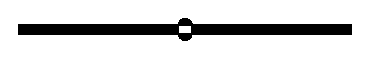
\includegraphics[width=2.5cm]{./images/affine_with_doubled_origin2.eps} / a field $k$.}
    $k$ :: field,
    $X$ :: affine with doubled origin /$k$とする.
    より詳細に,$X$は$X_1=\Spec k[x_1], X_2=\Spec k[x_2]$を
    $U_1=X_1-\{O_1\}, U_2=X_2-\{O_2\}$で貼りあわせたものとする.
    ただし$O_1 \in X_1,O_2 \in X_2$は原点である.
    $X_i, U_i, O_i ~~(i=1,2)$はすべて$X$の部分集合とみなす.
    また$U=X_1 \cap X_2=X-\{O_1, O_2\}$とする.
    明らかに$U=U_1=U_2 \iso \affine^1-\{0\}=\Spec k[x_1, x_1^{-1}]$.
    また$x_1|_U=x_2|_U$.

    \paragraph{Plot.}
    まず,$X$上のinvertible sheaf全体$\Pic X$がどのようなものか調べる.
    これは$\Pic X \iso \Z$となる.
    $n \in \Z$に対応する$\Pic X$の元を$\shL_n$とする.
    次に,generated by global sectionであるようなinvertible sheafを考える.
    これは$\shL_0(=\shO_X)$しかない.
    すると任意の$m>0, n \neq 0$について
    \begin{align*}
        \shL_0 \otimes (\shL_n)^{\otimes m} &= \shL_{mn} \neq \shL_0. \\
        \shL_n \otimes (\shL_0)^{\otimes m} &= \shL_n \hspace{7pt}\neq \shL_0.
    \end{align*}
    なので,どのinvertible sheafもampleでない.

    \paragraph{$X$ :: noetherian integral scheme.}
    $X_1, X_2 \iso \affine^1=\Spec k[x_1]$とreducedがlocalな性質であることから
    $X$ :: noetherian reduced scheme.
    $X$ :: irreducibleも明らかだから,
    $X$ :: noetherian integral scheme.

    \paragraph{$\Pic X \ni \shL=\shL(D)$.}
    $\shL \in \Pic X$を任意にとる.
    $X$ :: integralとProp6.15より,
    $\shL=\shL(D)$となる$D \in \CaCl X$が存在する.
    Prop6.13の証明から$D$がどのような形のものか考えよう.
    Example 6.3.1, Cor 6.16より,$\Pic X_1, \Pic X_2$.
    なので$\shL|_{X_1} \iso \shO_{X_1}, \shL|_{X_2} \iso \shO_{X_1}$となる.
    Prop6.13の証明から,$D$は次のような形をしている.
    \[
        D=\{ \sect{X_1}{f_1}, \sect{X_2}{f_2} \}
        \mwhere
        f_1 \in \Gamma(X_1, \shK_{X_1}^*)=(k(x_1))^*,
        f_2 \in \Gamma(X_2, \shK_{X_2}^*)=(k(x_2))^*.
    \]

    \paragraph{$D \sim \{ \sect{X_1}{x_1^n}, \sect{X_2}{1} \}$.}
    Cartier divisorの定義から,
    $U=X_1 \cap X_2$において$f_1/f_2 \in \Gamma(U, \shO_U^*)$となっている.
    $U \subseteq X_1=\Spec k[x_1]$と考えると,
    $U=\Spec k[x_1]_{x_1}=\Spec k[x_1, x_1^{-1}]$.
    ($U \subseteq X_1$と見れば$U=\Spec k[x_2,x_2^{-1}]$であるが,どちらでも同じである.)
    そして
    \[ \Gamma(U, \shO_U^*)=(k[x_1, x_1^{-1}])^*=\{ \alpha x_1^{n} \mid \alpha \in k^*, n \in \Z \}. \]
    であるから,$f_1/f_2=\alpha x_1^{n} (\iff f_2/f_1=(\alpha x_2^n)^{-1})$と書ける.
    よって
    \[
        D
        =\{ \sect{X_1}{\alpha x_1^n f_2}, \sect{X_2}{f_2} \}
        \mwhere
        f_2 \in \Gamma(X_2, \shK_{X_2}^*)=(k(x_2))^*.
    \]
    再び$X$ :: integralから,$\shK_X$はconstant sheafであり,
    したがって$f_2 \in K=\Gamma(X, \shK_X^*)$となる.
    なので
    $\{ \sect{X_1}{f_2}, \sect{X_2}{f_2} \}$はprincipal.
    加えて$\{ \sect{X_1}{\alpha}, \sect{X_2}{1} \} \in \Gamma(X, \shO_X^*)$なので
    \footnote
    {
        ここの部分はProp6.13cを用いて
        \[
            \shL(\{ \sect{X_1}{\alpha}, \sect{X_2}{1} \})
            =\shO_X
            =\shL(\{ \sect{X_1}{1}, \sect{X_2}{1} \})
        \]
        故に
        $\{ \sect{X_1}{\alpha}, \sect{X_2}{1} \}
            =\{ \sect{X_1}{1}, \sect{X_2}{1} \}$,
        と理解しても良い.

    },
    結局$D \sim \{ \sect{X_1}{x_1^n}, \sect{X_2}{1} \}$.

    \paragraph{$\Pic X \iso \Z$.}
    $n \in \Z$に対し,次のように定める.
    \[ D_n=\{ \sect{X_1}{x_1^n}, \sect{X_2}{1} \},~~~ \shL_n=\shL(D_n). \]
    これは次の写像を定める.
    \begin{defmap}
        {}& \Z& \to& \CaCl X \\
        {}& n& \mapsto& D_n
    \end{defmap}
    明らかに$D_m+D_n=D_{m+n}, \shL_m \otimes \shL_n=\shL_{m+n}$だから,
    これは加法群としての全射準同型.
    最後に,単射であることを見よう.
    $D_n=D_0$ならば,$D_0$同様$D_n$もprincipalである.
    したがって次を満たす$f \in \Gamma(X, \shK_X^*)$が存在する.
    \[
        f|_{X_1}/x_1^n \in \Gamma(X_1, \shO_{X_1}^*)=k^*,~~~
        f|_{X_2}/1 \in \Gamma(X_2, \shO_{X_2}^*)=k^*
    \]
    ここから$f|_{X_1} \in k^*$が得られる.
    よって$(f|_{X_1})/x_1^n \in k^*$と合わせて$n=0$を得る.
    このことは次の段落でも使うので,別に主張として述べておく.

    \begin{Claim}
        $f \in \Gamma(X, \shK_X^*)$とする.
        $f|_{X_2} \in k^*$ならば,$f|_{X_1} \in k^*$.
    \end{Claim}
    \begin{proof}
        $f|_{X_2} \in k^*$から$f|_U \in k^*$が得られる.
        $f|_U=\alpha$としよう.
        $U=\Spec k[x_1]_{x_1} \subset X_1$をみなして考えると,
        $k[x_1]_{x_1}$の元として$(f|_{X_1})|_U=\alpha$となっている.
        なので整数$r \geq 0$が存在し,
        $k[x_1]$の元として$x_1^r(f|_{X_1}-\alpha)=0$.
        しかし$k[x_1]$は整域なので,結局$f|_{X_1}=\alpha \in k^*$.
    \end{proof}

    \paragraph{Globally Generated Invertible Sheaf on $X$.}
    $n \in \Z$を任意にとり,
    $\{g_i\}_i \subseteq \Gamma(X, \shL_n)$が$\shL_n$のglobal generatorsであるとしよう.
    $\shL_n=\shL(D_n)$だから,
    $\shL_n|_{X_1}$は$x_1^n$でgenerateされ,
    $\shL_n|_{X_2}$は$1$でgenerateされている.
    特に後者から,$\shL_n|_{U}$は$1$でgenerateされている.
    したがってstalkで見れば,次のようになっている.
    \begin{align*}
        \Forall{P \in X_2}
        &\langle \{(g_i)_{P}\}_i \rangle
            \hspace{3.5pt}
            =(\shL_n)_{P}
            \hspace{3.7pt}
                =\shO_{X, P}
                    &&\text{  as  $\shO_{X, P}$-module.} \\
        &\langle \{(g_i)_{O_1}\}_i \rangle_i
            =(\shL_n)_{O_1}
                =(x_1^n)_{O_1} \shO_{X, O_1}
                    &&\text{  as  $\shO_{X, O_1}$-module.}
    \end{align*}
    これらを可換環に翻訳し,
    $g_i$を$g_i|_{X_2}, g_i|_U, g_i|_{X_1}$の順に求めていく.
    $X_2=\Spec k[x_2]$だから,
    $P$に対応する素イデアル$\I{p} \subset k[x_2]$がとれる.
    また,$g_i|_{X_2} \in \Gamma(X_2, \shO_X)=k[x_2]$.
    $\shO_{X,P}=\shO_{X_2, P}=k[x_2]_{\I{p}}$であり,
    したがって$k[x_2]_{\I{p}}$-moduleとして
    $\langle (g_i|_{X_1})_{\I{p}} \rangle=k[x_2]_{\I{p}}$.
    なので,次が成り立つ.
    \[
        \Forall{\I{p} \in \Spec k[x_2]} \Forall{i}
        (g_i|_{X_2})_{\I{p}} \in (k[x_2]_{\I{p}})^*=k[x_2] \setminus \I{p}.
    \]
    よって$g_i|_{X_2} \in (k[x_2])^*=k^*$がわかる.
    前段落に書いた主張から$g_i|_{X_1} \in k^*$.
    $\langle (g_i)_{O_1} \rangle_i=(x_1^n)_{O_1} \shO_{X, O_1}$
    と合わせて$(g_i|_{X_1})/x_1^{n} \in k^*$が得られ,$n=0$となる.
    以上より,$\shL_0$のみがgenerated by global sectionsである.

    \paragraph{Another Proof: Globally Generated Invertible Sheaf on $X$.}
    $n \in \Z$をとり,
    $\{g_i\}_i \in \Gamma(X, \shL_n)$を$\shL_n$のglobal generatorとする.
    $\shL_n|_{X_1}$は$x_1^n$で,$\shL_n|_{X_2}$は$1$で生成されており,
    $X_1, X_2$共にaffine schemeである.
    そのため,次のようになる.
    \begin{align*}
        &\langle \{ g_i|_{X_2} \}_i \rangle
            =\Gamma(X_2, \shL_n|_{X_2})
               =k[x_2]
                    &&\text{  as  $k[x_2]$-module.} \\
        &\langle \{ g_i|_{X_1} \}_i \rangle
            =\Gamma(X_1, \shL_n|_{X_1})
                =x_1^n k[x_1]
                    &&\text{  as  $k[x_1]$-module.}
    \end{align*}
    一行目から,$\{g_i|_{X_2}\} \subseteq (k[x_2])^*=k^*$.
    なので前々段落の主張から,$\{g_i|_{X_1}\} \subseteq k^*$.
    よって$x_1^n \in (k[x_1])^*=k^*$が得られる.

    \paragraph{資料.}
    詰まったところでは次のページを参考にした:
    \url{ https://math.stackexchange.com/questions/70042 }.
          
\section{Ample and Very Ample are Inherted by Tensor Products.} %% Ex7.5 
    $X$ :: noetherian scheme,
    $\shL, \shM$ :: invertible sheaves on $X$
    とする.
    \textbf{``generated by global sections"はgbgsと略す.}
    (d), (e)では更に
    $X$ :: finite type over a noetherian ring $A$,と仮定する.
    (これはThm7.6の仮定である.)

    \begin{Lemma}
        If $\shM, \shM'$ :: gbgs invertible sheaves on $X$,
        then $\shM \otimes_{\shO_X} \shM'$ :: gbgs.
    \end{Lemma}
    \begin{proof}
        $\{m_i\} \subseteq \Gamma(X, \shM), \{m'_j\} \subseteq \Gamma(X, \shM')$を
        それぞれ$\shM, \shM'$のglobal generatorとする.
        定義より,このことは次と同値である:
        任意の点$x \in X$について$\shM_x, \shM'_x$はそれぞれ
        $\{(m_i)_x\}_i, \{(m'_i)_x\}_j$で$\shO_{X,x}$-moduleとして生成される.
        さて,tensor productはleft adjointであることからcolimitと交換する.
        なので$(\shM \otimes_{\shO_X} \shM')_x$は
        $\shM_x \otimes_{\shO_{X,x}} \shM'_x$と同型である.
        明らかにこれは$\{(m_i)_x \otimes (m'_i)_x\}_{i,j}$で生成される
        (Ati-Mac \S2.7)から,$\shM \otimes_{\shO_X} \shM'$ :: gbgs.
        global generatorは$\{m_i \otimes m'_i\}_{i,j}$である.
    \end{proof}

    \subsection{If $\shL$ :: ample and $\shM$ :: gbgs then $\shL \otimes \shM$ :: ample.}
        $\shF$ :: coherent sheaf on $X$とする.
        $\shL$ :: ampleなので,十分大きな$n>0$について
        $\shF \otimes \shL^{\otimes n}$ :: gbgs.
        これに$\otimes \shM^{\otimes n}$を合わせて整理すると,
        補題から$\shF \otimes (\shL \otimes \shM)^{\otimes n}$ :: gbgs.
        よって$\shL \otimes \shM$ :: ample.

    \subsection{If $\shL$ :: ample and $\shM$ :: arbitrary
        then $\shM \otimes \shL^{\otimes n}$ :: ample for some $n>0$.}
        $\shM$ :: coherentなので,十分大きな$n>0$について
        $\shM \otimes \shL^{\otimes n}$ :: gbgs.
        任意の$\shF$ :: coherent sheafに対して十分大きい$r>0$をとると,
        $\shF \otimes \shL^{\otimes rn}$ :: gbgs.
        補題より次もgbgs:
        \[ (\shF \otimes \shL^{\otimes rn}) \otimes (\shM \otimes \shL^{\otimes n})^{\otimes r}. \]
        整理して$\shF \otimes (\shM \otimes \shL^{\otimes 2n})^{\otimes r}$ :: gbgs.
        よって$\shM \otimes \shL^{\otimes 2n}$ :: ample.

    \subsection{If $\shL, \shM$ :: ample then $\shL \otimes \shM$ :: ample.}
        $\shF$ :: cohenrent sheaf on $X$とする.
        十分大きな$l>0$について,$\shF \otimes \shL^{\otimes l}$ :: gbgs.
        このsheafもcoherentなので,十分大きな$m>0$について
        $\shF \otimes \shL^{\otimes l} \otimes \shM^{\otimes m}$ :: gbgs.
        $n=\max(l,m)$とすれば
        $\shF \otimes \shL^{\otimes n} \otimes \shM^{\otimes n}$ :: gbgs.
        整理すれば$\shL \otimes \shM$ :: ampleが得られる.

    \subsection{If $\shL$ :: very ample and $\shM$ :: gbgs then $\shL \otimes \shM$ :: very ample.}
    $\shL, \shM$に対応するmorphismを,
    それぞれ$i: X \to \proj^m_A, j: X \to \proj^n_A$とする.
    Thm7.1bより,$\shL \iso i^* \shO(1), \shM \iso j^* \shO(1)$.
    この時,次の(1)のような$2$重のfiber productを考える.
    ここでの$\proj^N$は$\proj^m, \proj^n$のCartesian product(Ex5.11)であり,
    $N=mn+m+n$である.
    \[
        (1)
        \xymatrix@C=12pt
        {
            {} & {} & {} & {} \\
            {} & X \times_A X \ar[rr]\ar[dd]\ar[rd]^-{i \times j}& {} &  X \ar[d]^-{i} \\
            {} & {} & \proj^{N}_A \ar[r]^-{p_1}\ar[d]_-{p_2}& \proj^m_A \ar[d] \\
            {}& X \ar[r]_-{j}& \proj^n_A \ar[r]& \Spec A
        }
        \hspace{40pt}
        (2)
        \xymatrix@C=12pt
        {
            X \ar@{=}[rrr]\ar@{=}[ddd]\ar@{->}[rrdd]^(.7){\omega}& {} & {} &  X \ar@{=}[d]\\
            {} & X \times_A X \ar[rr]\ar[dd]& {} &  X \ar[d]^-{i} \\
            {} & {} & \proj^{N}_A \ar[r]^-{p_1}\ar[d]_-{p_2}& \proj^m_A \ar[d] \\
            X \ar@{=}[r]& X \ar[r]_-{j}& \proj^n_A \ar[r]& \Spec A
        }
    \]
    (2)では$X$を図式に付け加え,
    fiber product $X \times X$の普遍性から誘導される射と$i \times j$の合成を$\omega$としている.
    $\omega^*\shO_{\proj^N}(1)$を計算すると,次のようになる.
    \begin{align*}
        {}&     ~\omega^*\shO_{\proj^N}(1) \\
        \iso&   ~\omega^* (p_1^* \shO_{\proj^m}(1) \otimes_A p_2^* \shO_{\proj^m}(1)) \\
        \iso&   ~\omega^* p_1^* \shO_{\proj^m}(1) \otimes_A \omega^* p_2^* \shO_{\proj^m}(1) \\
        \iso&   ~(p_1 \circ \omega)^* \shO_{\proj^m}(1) \otimes_A (p_2 \circ \omega)^* \shO_{\proj^m}(1) \\
        \iso&   ~i^* \shO_{\proj^m}(1) \otimes_A j^* \shO_{\proj^m}(1) \\
        \iso&   ~\shL \otimes_A \shM
    \end{align*}
    上から順に,
    Ex5.11,
    Ex5.1の解答にある補題,
    $(p_{-} \circ \omega)_*$が$\omega^* p_{-}^*$にadjointであること
    \footnote
        {
            もう少し詳しく述べておこう.
            $X \xrightarrow{f} Y \xrightarrow{g} Z$を考える.
            $f^* g^*$は$g_* f_*=(g \circ f)_*$とadjoint.
            そして$(g \circ f)_*$は$(g \circ f)^*$とadjoint.
            これとadjointの一意性から$f^* g^* \iso (g \circ f)^*$が得られる.
        },
    図式の可換性を用いている.
    最後に$\omega$がimmersionであることを示そう.
    \begin{Claim}
        $i: X \to \proj^m_A$をimmersionとする.
        次の可換図式において,$X \to \proj^N_A$はimmersionである.
        \[
        \xymatrix@R=35pt@C=15pt
        {
            X \ar@{=}[rrr]\ar@{=}[ddd]\ar[rd]& {} & {} &  X \ar@{=}[d]\\
            {} & X \times_A X \ar[rd] \ar[r]\ar[d]& \proj^N \times X \ar[r]\ar[d]&  X \ar[d]^-{i} \\
            {} & X \times \proj^N \ar[d]\ar[r]& \proj^{N}_A \ar[r]^-{p_1}\ar[d]_-{p_2}& \proj^m_A \ar[d] \\
            X \ar@{=}[r]& X \ar[r]_-{j}& \proj^n_A \ar[r]& \Spec A
        }
        \]
    \end{Claim}
    \begin{proof}
        (TODO)
        多分示す必要があるもの:
        $j, X \to X \times X$ :: closed immersion,
        immersion :: stable under base extension \& inherted by composition.
        以上を示すと,主張は自明になる.
        $j$ :: closed immersionはProp7.2とThm7.6の証明から得られると思う.
        $X \to X \times X$ :: closed immersionは
        $X \times X$との合成がsurjectiveであることから,
        定義にしたがって示せると思う.
    \end{proof}

    \subsection{If $\shL$ :: ample then $\shL^{\otimes n}$ :: very ample for sufficiently large all $n>0$.}
    Thm7.6より,ある正整数$l>0$について$\shL^{\otimes l}$ :: very ample.
    また,$\shL$ :: ampleより,
    正整数$m_0>0$が存在し,
    任意の整数$m \geq m_0$について$\shO_X \otimes \shL^{\otimes m}$ :: gbgs.
    したがって,$N=n+m_0$とおけば,(d)より
    \[ (\shO_X \otimes \shL^{\otimes m}) \otimes \shL^{\otimes l}=\shL^{\otimes n} ~~~ (m \geq m_0, n \geq N) \]
    はvery ampleである.

\section{The Riemann-Roch Problem.} %% Ex7.6 
    $k$ :: algebraically closed field,
    $X$ :: nonsingular projective variety over $k$,
    $D$ :: divisor on $X$
    とする.
    (したがって$|D|$ :: linear systemが考えられる.)
    この時,$n$の関数$\dim_k |nD|$を考える.
    $\shL$を$D$に対応するinvertible sheafとすると,
    Prop7.7より,これは$\dim_k \Gamma(X, \shL^n)-1$とも書ける.

    Ex2.14とCor5.16を合わせると,
    $X=\Proj k[x_0, \dots, x_d]/I$なる$I$ :: homogeneous idealが
    存在することが分かる.
    そこで$S=k[x_0, \dots, x_d], T=S/I$としておく.
    また$\phi: S \to T=S/I$を標準的全射としておく.

    \subsection{$D$ :: very ample $\implies \Forall{n \gg 0} \dim_k |nD|=P_X(n)-1$.}
    今,$\shL$ :: very ampleだから,
    $i^* \shO_{\proj^d}(1) \iso \shL$となる
    closed immersion $i: X \to \proj^d_k$が存在する.
    (closedであることはRemark5.16.1と同様.)
    Ex6.8a($i^*$と$\otimes$が分配的であること)とProp5.12(の証明)から次が分かる.
    \[
        \shL^{\otimes n}
        =(i^* \shO_{\proj^d}(1))^{\otimes n}
        \iso i^* ((\shO_{\proj^d}(1))^{\otimes n})
        \iso i^* (S(n) \sidetilde)
        \iso (S(n) \otimes T)\sidetilde.
    \]
    $\phi$が次数を保つこと(したがって$\phi(S(n))=T(n)$)から,
    $S(n) \otimes T \iso T(n)$.
    Ex5.9bより,十分大きい全ての$n$について$T_n \iso \Gamma(X, (T(n))\sidetilde)$となる.
    よって,
    $P_X$を$X$のHilbert polynomialとすると,
    十分大きい全ての$n$について$P_X(n)=\dim_k \Gamma(X, \shL^{\otimes n})$.

    \subsection{If $D$ is torsion element of order $r$,
        then $\dim_k |nD|=0$ if $r \divible n$ \& $=-1$ otherwise}

    orderの定義から,$nD=0 \iff n \bmod r=0$であることに注意する.
    次を示す.
    \[
        \dim_k |nD|=
        \begin{cases}{}
            0   & n \bmod r=0 \\
            -1  & n \bmod r \neq 0
        \end{cases}
    \]

    \paragraph{$n \bmod r=0 \implies \dim_k |nD|=0$.}
    $n \bmod r=0$の時,$nD=0$,$\shL^{\otimes n}=\shO_X$.
    今,$X$ :: integral \& proper \& finite type scheme over algebraically closed subset.
    なのでEx4.5dより,$\Gamma(X, \shO_X)=k$.
    よって$\dim_k |nD|=\dim_k \Gamma(X, \shO_X)-1=0$.

    \paragraph{$n \bmod r \neq 0 \implies |nD|=\emptyset \implies \dim_k |nD|=-1$.}
    $n \bmod r \neq 0$の時,$|nD|=\emptyset$を示す.
    $E=\{\sect{U_i}{f_i}\}_i \in |nD|$がとれるとして矛盾を導くことにする.
    $E$ :: effectiveかつ$E \sim nD \not \sim 0$なので,
    $f_i \in \Gamma(U_i, \shO_{U_i})$は単元でない.
    したがって$f_i^r$も単元でない
    \footnote
    {
        $f_i$は単元でないから,$\Gamma(U_i, \shO_{U_i})$の真のイデアルに属す.
        そして$f_i^r$もこのイデアルに属し,
        したがって$f_i^r$は単元でない.
    }.
    いずれの$i$についても同様なので,
    $rE$はprincipalでない($rE \not \sim 0$).
    一方,$E \sim nD, rD=0$だから$rE \sim rnD \sim 0$.

\section{Some Rational Surfaces.} %% Ex7.7 

\section{Sections of $\pi: X \to \pbundle(\shE)$
    $\leftrightarrow$ Quotient Invertible Sheaves of $\shE$.} %% Ex7.8 

    $X$ :: noetherian scheme,
    $\shE$ :: coherent locally free sheaf on $X$とする.
    Prop7.12において$Y=X, g=\id{X}$とすると,
    以下の図式を成立させる$\sigma: X \to \pbundle(\shE)$と
    quotient invertible sheaf of $\shE $:: $\shE \to \shL \to 0$が
    \footnote
    {
        $\shE \to \shL \to 0$だけで$\shL$と全射 :: $\shE \to \shL$の組を意味する.
        $g^*\shE=\shE$に注意.
    }
    対応することがわかる.
    \[
        \xymatrix
        {
            X \ar[r]^-{\sigma}\ar[d]_-{\id{X}}& \pbundle(\shE) \ar[ld]^-{\pi} \\
            X
        }
    \]
    明らかに$\sigma$は$\pi$のsectionである.

\section{$\Pic \pbundle(\shE) \iso \Pic X \times \Z$.} %% Ex7.9 
    $X$ :: regular noetherian scheme,
    $\shE$ :: locally free coherent sheaf of rank $\geq 2$ on $X$とする.
    $r=\rank \shE (\geq 2)$とおく.

    \subsection{$\Pic \pbundle(\shE) \iso \Pic X \times \Z$.}
    $X$はlocally factorial, reduced, noetherian schemeである.
    Prop4.1よりaffine schemeはseparatedだから,
    $X$の任意のirreducible affine open subset :: $U=\Spec A$はCor6.16の条件を満たす.
    したがって$\Pic U \iso \Cl U$.
    そしてp.162から$\pi^{-1}(U) \iso \proj^{r-1}_A$.
    
    Ex7.8の図式から,次のsplitする図式が得られる.
    \[
        \xymatrix
        {
            0 \ar[r]& \ker \sigma^* \ar[r]& \Pic \pbundle(\shE) \ar@<2pt>[r]^-{\sigma^*}&\ar@<2pt>[l]^-{\pi^*} \Pic X \ar[r]& 0
        }
    \]

    \subsection{$\pbundle(\shE) \iso \pbundle(\shE') \iff
        \Exists{\shL \in \Pic X} \shE'=\shE \otimes \shL$.}
    $\shE'$ :: locally free coherent sheaf on $X$とする.
    ($\rank \shE' \geq 2$という条件はついていない.)

\section{$\proj^n$-Bundles Over a Scheme.} %% Ex7.10 

\section{Different Sheaves of Ideals can Give Rise to Isomorphic Blow Up Schemes.} %% Ex7.11 

\section{ } %% Ex7.12 

\section{* A Complete Nonprojective Variety.} %% Ex7.13 

\section{ } %% Ex7.14 


\end{document}
